\documentclass[a4paper,11pt]{report}
 
 \usepackage[left=3cm, right=3cm, top=3cm, bottom=3cm]{geometry}
\usepackage{graphicx}
\usepackage{listings}
\usepackage{titlesec}
\usepackage{fancyhdr}
\usepackage{epstopdf}
\usepackage{float}
\usepackage{amsmath}
\usepackage{setspace}
\usepackage{eufrak}
\usepackage{url}

\usepackage{courier}
 \newcommand{\textform}[1]{\fontsize{14}{20}\selectfont{#1}}
\pagestyle{fancy}
\fancyhf{}
\fancyhead[R]{\thepage}
\renewcommand{\chaptermark}[1]{\markboth{#1}{}}
\renewcommand{\headrulewidth}{1pt}
\renewcommand{\footrulewidth}{1pt}

\lhead{\footnotesize{FLIPPER ZERO
}}
\rhead{}
\lfoot{\footnotesize{Department of Computer Science \& Engg.}}
\cfoot{}
\rfoot{\thepage}

\titleformat{\chapter}[display]
{\normalfont\Large\bfseries\centering}{\chaptertitlename\
\thechapter}{20pt}{\Large}


%\title{\textbf{A seminar report on\\TRUSTWORTHINESS MANAGEMENT IN THE SOCIAL INTERNET OF THINGS} 
%}
%\author{\textbf{Deena Jose}}

\begin{document}

\thispagestyle{empty}
  \begin{center}
      \fontsize{22}{25}\selectfont{\textbf{GOVERNMENT POLYTECHNIC COLLEGE PERUMBAVOOR}}\\[.1cm]
            \fontsize{15}{25}\selectfont{\textbf{Koovappady P.O Ernakulam-683 544 Kerala
    }}\\[1.2cm]
    \begin{figure}[h]
	\centering
	\hspace{21pt}
	
\includegraphics[width=.70\linewidth]{logo.png}
	\label{fig:logo.png}
\end{figure}
\fontsize{14}{25}\selectfont{\textbf{Semester - VI}}\\
\fontsize{14}{25}\selectfont{\textbf{Computer Engineering 2022-23}}\\[.8cm]

    \fontsize{14}{25}\selectfont{\textbf{A SEMINAR REPORT}}\\[.1cm]
    \fontsize{14}{25}\selectfont{on}\\
    \fontsize{20}{25}\selectfont{\textbf{FLIPPER ZERO
    }}\\[1.2cm]
    \end{center}
    \begin{minipage}{.4\textwidth}
    \begin{flushleft}
    \begin{center}
    \fontsize{12}{25}\selectfont{\textbf{Submitted by}}\\[.2cm]
    \fontsize{14}{25}\selectfont \bfseries{MANU MOHAN}\\[.1cm]
    \fontsize{12}{25}\selectfont{\textbf{manumm9526@gmail.com}}\\[.2cm]
%\vfill
 \end{center}
    \end{flushleft}
      \end{minipage}
\begin{minipage}{0.8\textwidth}
\begin{flushright}
\begin{center}
    \fontsize{12}{25}\selectfont{\textbf{Lecturer}}\\[.2cm]
%\vfill
\fontsize{14}{25}\selectfont \bfseries{IVY BALAN}\\[.1cm]
\fontsize{12}{25}\selectfont{\textbf{balanivy@gmail.com}}\\[.2cm]
\end{center}
\end{flushright}
\end{minipage}

\fontsize{12pt}{20}\selectfont
\thispagestyle{empty}
 


\thispagestyle{empty}
  \renewcommand\abstractname{\textform{\textbf{ABSTRACT}}}
    \begin{abstract}
      \vspace{1.0cm}

 \paragraph{ }Flipper Zero is a highly versatile and portable device designed for security testing and digital forensics. It is an open-source device, which means that it can be highly customized and adapted to specific tasks and requirements. Its range of tools and capabilities, including wireless protocol analysis and hardware interface testing, make it an ideal tool for security professionals and digital forensic investigators.
 

 The device is highly intuitive and easy to use, with a simple interface that can be navigated by both novice and experienced users. Its portability is another advantage, making it easy to take on the go and use in a variety of settings. It can also be customized with additional functionality through the use of open-source software and hardware add-ons.
 
 However, as with any technology, there are also some limitations and potential vulnerabilities associated with Flipper Zero. Its hardware capabilities may be limited compared to more specialized tools, and there may be a learning curve for new users. As an open-source device, it relies on ongoing support and contributions from the community to remain up-to-date and secure.
\end{abstract}

  \tableofcontents
\thispagestyle{empty}

\chapter{INTRODUCTION}

\paragraph{}Flipper Zero is a versatile and portable device that is designed for security testing and digital forensics. It offers a range of tools and capabilities, including wireless protocol analysis, RFID scanning, and hardware interface testing. Its open-source design and customizable nature make it an ideal tool for security professionals and digital forensic investigators who are looking for a flexible and adaptable device.

The device's ease of use and portability are also significant advantages. It is designed with a simple and intuitive interface that can be navigated by both novice and experienced users. Its small and lightweight design also makes it easy to take on the go and use in a variety of settings.

Despite its many advantages, it is important to be aware of the potential limitations and vulnerabilities associated with the device. As an open-source device, it relies on ongoing support and contributions from the community to remain up-to-date and secure. Additionally, its hardware capabilities may be limited compared to more specialized tools, and there may be a learning curve for new users.

Overall, Flipper Zero is a cost-effective and flexible solution for security testing and digital forensics. Its range of tools and capabilities, combined with its ease of use and portability, make it an ideal tool for those looking for a versatile and customizable device.
  
\chapter{KEY FEATURES OF FLIPPER ZERO}
Homomorphic encryption has been the subject of research for several decades, with many different approaches proposed. One of the earliest proposals for homomorphic encryption was by Rivest, Adleman, and Dertouzos in 1978, who proposed the concept of "privacy homomorphisms" . Since then, a large body of research has been conducted on the topic, including the development of various homomorphic encryption schemes, such as fully homomorphic encryption and partially homomorphic encryption.
\begin{figure}[h]
	\centering
	\hspace{21pt}
	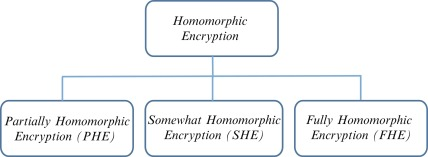
\includegraphics[width=.70\linewidth]{type.jpg}
	\label{fig:type.png}
\end{figure}
\section{Fully homomorphic encryption(FHE)}
Fully homomorphic encryption (FHE) is a type of homomorphic encryption that allows for arbitrary computations to be performed on encrypted data, without the need to decrypt the data beforehand. This has important implications for privacy and security, as sensitive data can be processed without revealing its underlying content. Gentry first proposed the concept of fully homomorphic encryption in 2009, using ideal lattices as the underlying mathematical structure [3]. Since then, further research has focused on improving the efficiency and practicality of FHE, and on the development of new FHE schemes.
\section{Partially homomorphic encryption(PHE)}\label{AA}
Partially homomorphic encryption (PHE), on the other hand, allows for a limited set of computations to be performed on encrypted data, such as addition or multiplication. This type of encryption is less computationally intensive than FHE, and is more practical for certain types of applications, such as data sharing and cloud computing.
  
\chapter{METHODOLOGY}

\section{Review of literature}
In conclusion, the field of homomorphic encryption has seen a great deal of research and development, with many different approaches proposed and evaluated.In addition to the development of different homomorphic encryption schemes, research has also focused on the efficiency of these algorithms. This includes the development of algorithms that minimize the number of encryptions and decryptions required, as well as the optimization of the underlying mathematical structures used in the encryption process. Despite these efforts, there are still many challenges to be addressed, including the efficiency of these algorithms, the development of practical and secure homomorphic encryption schemes, and the need for further research into the security and privacy implications of these techniques.
\begin{figure}[h]
	\centering
	\hspace{21pt}
	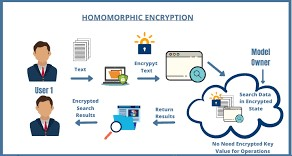
\includegraphics[width=.70\linewidth]{he.jpg}
	\label{fig:he.jpg}
\end{figure}
\section{Comparison of schemes}
Homomorphic encryption can be broadly categorized into two types: fully homomorphic encryption (FHE) and partially homomorphic encryption (PHE). Both types of homomorphic encryption have their own strengths and weaknesses, and are best suited for different applications.

Fully homomorphic encryption (FHE) allows for arbitrary computations to be performed on encrypted data, without the need to decrypt the data beforehand. This type of encryption offers the highest level of privacy, as sensitive data can be processed without revealing its underlying content. However, FHE is computationally intensive, and is less practical for many applications, due to its slow processing speed and large storage requirements.

Partially homomorphic encryption (PHE), on the other hand, allows for a limited set of computations to be performed on encrypted data, such as addition or multiplication. This type of encryption is less computationally intensive than FHE, and is more practical for certain types of applications, such as data sharing and cloud computing. However, PHE does not offer the same level of privacy as FHE, as it allows for certain computations to be performed on encrypted data, revealing some information about the underlying data.

In terms of security, both FHE and PHE offer strong security guarantees, as long as the underlying mathematical structures used in the encryption process are secure. However, FHE is generally considered to be more secure than PHE, as it allows for arbitrary computations to be performed on encrypted data, making it harder for an attacker to extract information about the underlying data.

In conclusion, the choice between FHE and PHE depends on the specific requirements of the application, including the level of privacy and security required, as well as the computational and storage requirements. For privacy-sensitive applications, such as medical data analysis or credit card fraud detection, FHE may be the preferred choice, as it offers the highest level of privacy. However, for applications that require fast processing and low storage requirements, PHE may be a more practical solution.
\section{Implementation of schemes}
For partial homomorphic encryption (PHE) schemes, the implementation typically involves the use of a public-key encryption system, such as RSA or ElGamal. The encryption process involves transforming the plaintext into ciphertext using the public key, and the decryption process involves transforming the ciphertext back into plaintext using the private key. For PHE schemes that allow for computations on encrypted data, such as addition or multiplication, specific algorithms are used to perform these computations on the ciphertext, without the need to decrypt the data beforehand.

For fully homomorphic encryption (FHE) schemes, the implementation typically involves the use of a lattice-based encryption system, such as the one proposed by Gentry in 2009. The encryption process involves transforming the plaintext into ciphertext using a set of parameters that define the underlying lattice structure, and the decryption process involves transforming the ciphertext back into plaintext using the private key. For FHE schemes, specific algorithms are used to perform arbitrary computations on the ciphertext, without the need to decrypt the data beforehand.

In terms of software implementation, homomorphic encryption schemes can be implemented using programming languages such as Python or C++. There are also several libraries and tools available that provide support for the implementation of homomorphic encryption, including the HElib library and the SEAL library.

In conclusion, the implementation of homomorphic encryption schemes can be a complex process, involving the use of complex mathematical algorithms and encryption systems. However, with the right tools and resources, it is possible to implement homomorphic encryption and gain the benefits of privacy and security for sensitive data.
\section{Encryption Algorithm}
Encryption algorithm is a mathematical process used to transform plaintext into ciphertext, making it unreadable to unauthorized parties. The encryption process is performed using an encryption key, which is a string of bits used to encrypt the data. The encryption key is kept secret, and is used to decrypt the ciphertext back into the original plaintext. There are several types of encryption algorithms, including symmetric-key algorithms, public-key algorithms, and hash functions. The choice of encryption algorithm depends on the specific requirements of the application, including the level of security required, the amount of data to be encrypted, and the computational resources available. Commonly used encryption algorithms include AES, RSA, and SHA-256.
example: AES (Advanced Encryption Standard) is a widely used symmetric-key encryption algorithm. It uses a fixed-size block cipher, which encrypts data in fixed-size blocks (128 bits), and operates on a fixed-size key (128, 192, or 256 bits). The encryption process involves transforming the plaintext into ciphertext using the encryption key and a set of fixed operations known as rounds. The decryption process involves reversing the encryption process, using the same encryption key, to transform the ciphertext back into the original plaintext.
 \begin{figure}[h]
	\centering
	\hspace{21pt}
	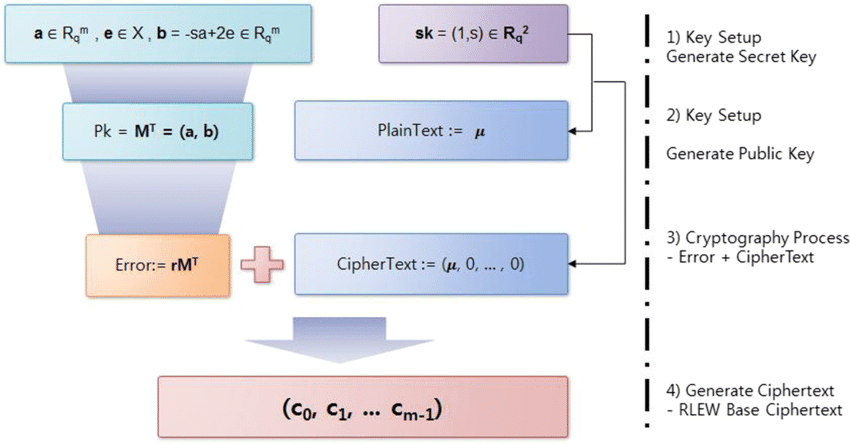
\includegraphics[width=.70\linewidth]{algo.png}
	\label{fig:type.png}
\end{figure}
\section{Security analysis}
\begin{itemize}
\item[•] Confidentiality: Confidentiality is the property that the encrypted data is kept secret from unauthorized parties. A security analysis of an encryption algorithm should determine the level of confidentiality provided by the algorithm and the conditions under which confidentiality is maintained.
\item[•] Integrity: Integrity is the property that the encrypted data has not been modified during transmission or storage. A security analysis of an encryption algorithm should determine the level of integrity provided by the algorithm and the conditions under which integrity is maintained.
\item[•] Availability: Availability is the property that the encrypted data is accessible when needed. A security analysis of an encryption algorithm should determine the level of availability provided by the algorithm and the conditions under which availability is maintained.

\item[•] Key size: Key size is an important factor in the security of an encryption algorithm. The larger the key size, the more secure the algorithm is considered to be. A security analysis of an encryption algorithm should determine the key size required to provide a desired level of security and the computational resources required to use the algorithm with that key size.

\item[•] Resistance to attacks: A security analysis of an encryption algorithm should determine the algorithm's resistance to various forms of attack, including brute-force attacks, known-plaintext attacks, and chosen-plaintext attacks.

\item[•] Efficiency: The efficiency of an encryption algorithm refers to the computational resources required to encrypt and decrypt data. A security analysis of an encryption algorithm should determine the efficiency of the algorithm and compare it to other algorithms.
\end{itemize}
 \begin{figure}[h]
	\centering
	\hspace{21pt}
	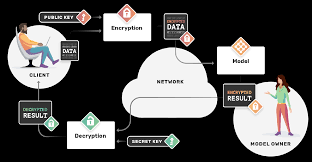
\includegraphics[width=.70\linewidth]{security.png}
	\label{fig:security.png}
\end{figure}
\section{Evaluation of Applications}
\begin{itemize}
\item[•] Security requirements: The security requirements of the application should be clearly defined, including the level of confidentiality, integrity, and availability required. The encryption algorithm should provide the necessary level of security to meet these requirements.

\item[•] Performance requirements: The performance requirements of the application should be taken into account, including the processing time required for encryption and decryption and the computational resources required. The encryption algorithm should be efficient enough to meet the performance requirements of the application.

\item[•] Key management: The key management system should be secure and efficient, and should support the use of multiple keys. The encryption algorithm should integrate well with the key management system and provide the necessary level of security for key management.

\item[•] Interoperability: The encryption algorithm should be interoperable with other encryption algorithms and with other systems. The encryption algorithm should be able to encrypt and decrypt data in a manner that is compatible with other encryption algorithms and with other systems.

\item[•] Cost: The cost of the encryption algorithm, including licensing and hardware costs, should be taken into account. The encryption algorithm should provide the necessary level of security at a cost that is acceptable to the user.

\item[•] Standards compliance: The encryption algorithm should comply with relevant standards and regulations, including national and international standards for encryption algorithms.
\end{itemize}

\chapter{CONCLUSIONS}
Homomorphic encryption is a powerful tool for privacy-preserving computation, and has the potential to revolutionize the way we store and process sensitive data. With further research and development, it is likely that this technology will become increasingly important in a variety of contexts, and will play a key role in ensuring the privacy and security of sensitive information.

\chapter{REFERENCES}

\begin{itemize}
\item[1] Stinson, D. R. (2005). Cryptography: theory and practice (Vol. 55). Boca Raton, FL: CRC press.
\item[2] Boneh, D.,Shacham, H. (2004). Group signatures with verifier-local revocation. In Proceedings of the 13th ACM conference on Computer and communications security (pp. 424-433).
\item[3] Menezes, A. J., van Oorschot, P. C.,  Vanstone, S. A. (1997). Handbook of applied cryptography. CRC press.
\item[4] Goldreich, O. (2001). Foundations of cryptography: basic tools. Cambridge University Press.
\item[5] Bellare, M., Rogaway, P. (1993). Optimal asymmetric encryption—how to encrypt with RSA. In Advances in Cryptology—CRYPTO'93 (pp. 92-111). Springer, Berlin, Heidelberg.

\vspace{12pt}
\end{itemize}
\end{document}
